\section{Results} \label{sec:Results}

The following are a series of our experimentations and results for particular
networks.

\subsection{Varying Training Steps}

We first examine the effect of number of training samples on the network. We can
look at the fully-connected (FC) network as a baseline and analyze the network's
configuration, which can be seen in \ref{fig:fcAdj}.

\begin{figure}[h]
    \centering
    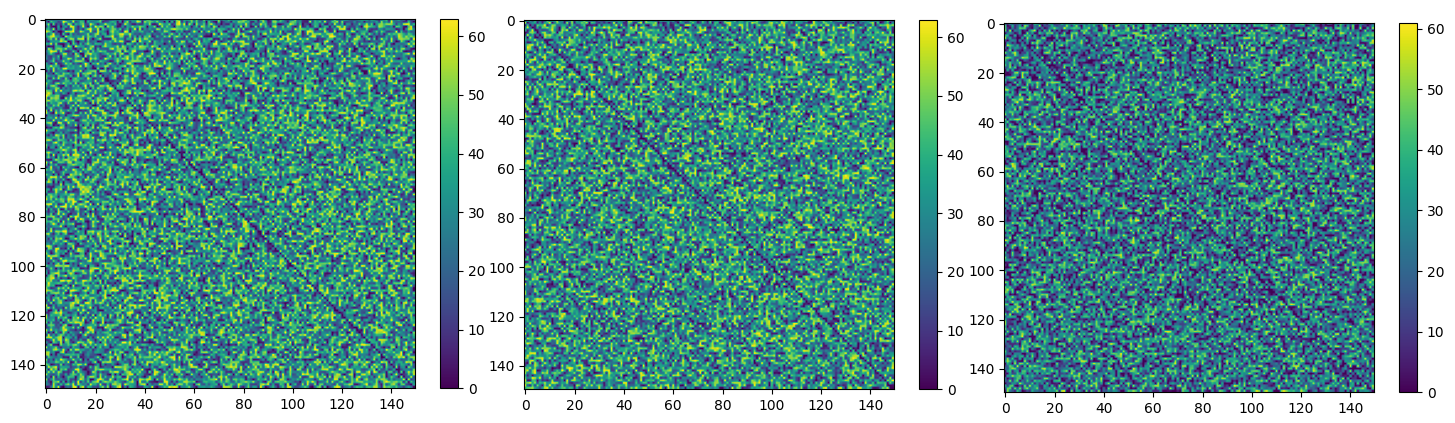
\includegraphics[scale=0.22]{fcAdj.png}
    \caption{
        Diagrams of the fully-connected network's adjacency matrices. The left
        diagram is at $n=10$ samples, the middle at $n=100$ samples, and the
        right at $n=1000$ samples.
    }
    \label{fig:fcAdj}
\end{figure}

Over larger training steps, the network's adjacency matrix becomes more
significantly sparse. We can pull out the difference matrices to further
elaborate this point in \ref{fig:fcAdjDiff}.

\begin{figure}[h]
    \centering
    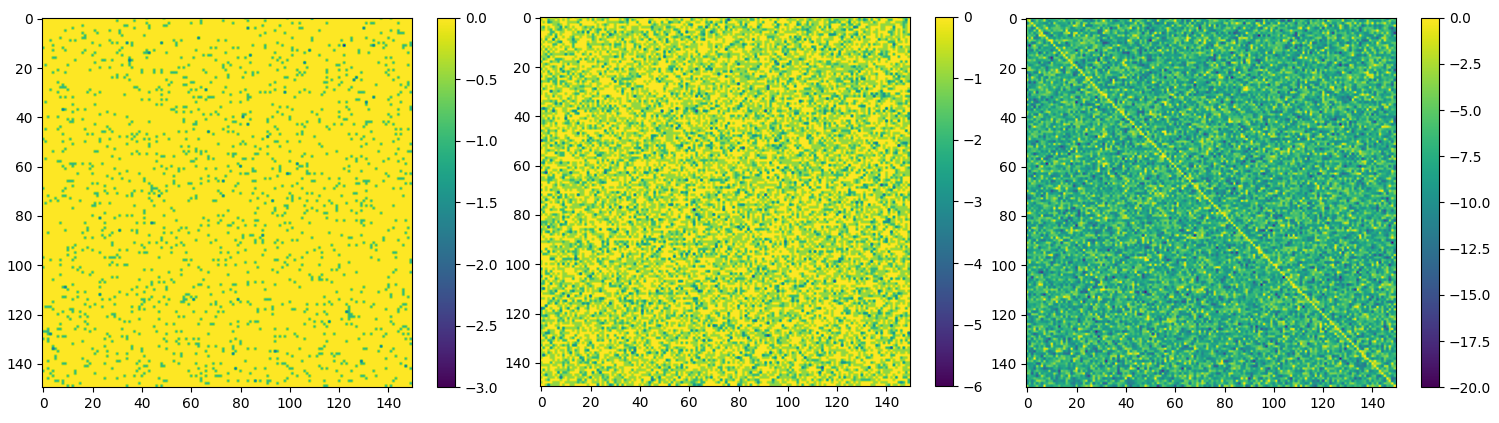
\includegraphics[scale=0.22]{fcAdjDiff.png}
    \caption{
        Diagrams of the fully-connected network's adjacency matrix differences
        from their initial seeds. The left diagram is at $n=10$ samples, the
        middle at $n=100$ samples, and the right at $n=1000$ samples.
    }
    \label{fig:fcAdjDiff}
\end{figure}

The matrices definitely get more sparse over time, despite extremely low $\mu_b$
backoff values. Networks are notably capable of building new connections, and
the connection removal parameter $\mu_b$ being very low indicates that the
network is still removing connections it deems 'unnecessary.' This tendency to
forget irrelevant information rapidly seems to be an underlying feature of STDP
training. This pattern repeats itself across a variety of networks, and can be
seen through the average degrees of all networks, in \ref{fig:avgDeg}.

\begin{figure}[h]
    \centering
    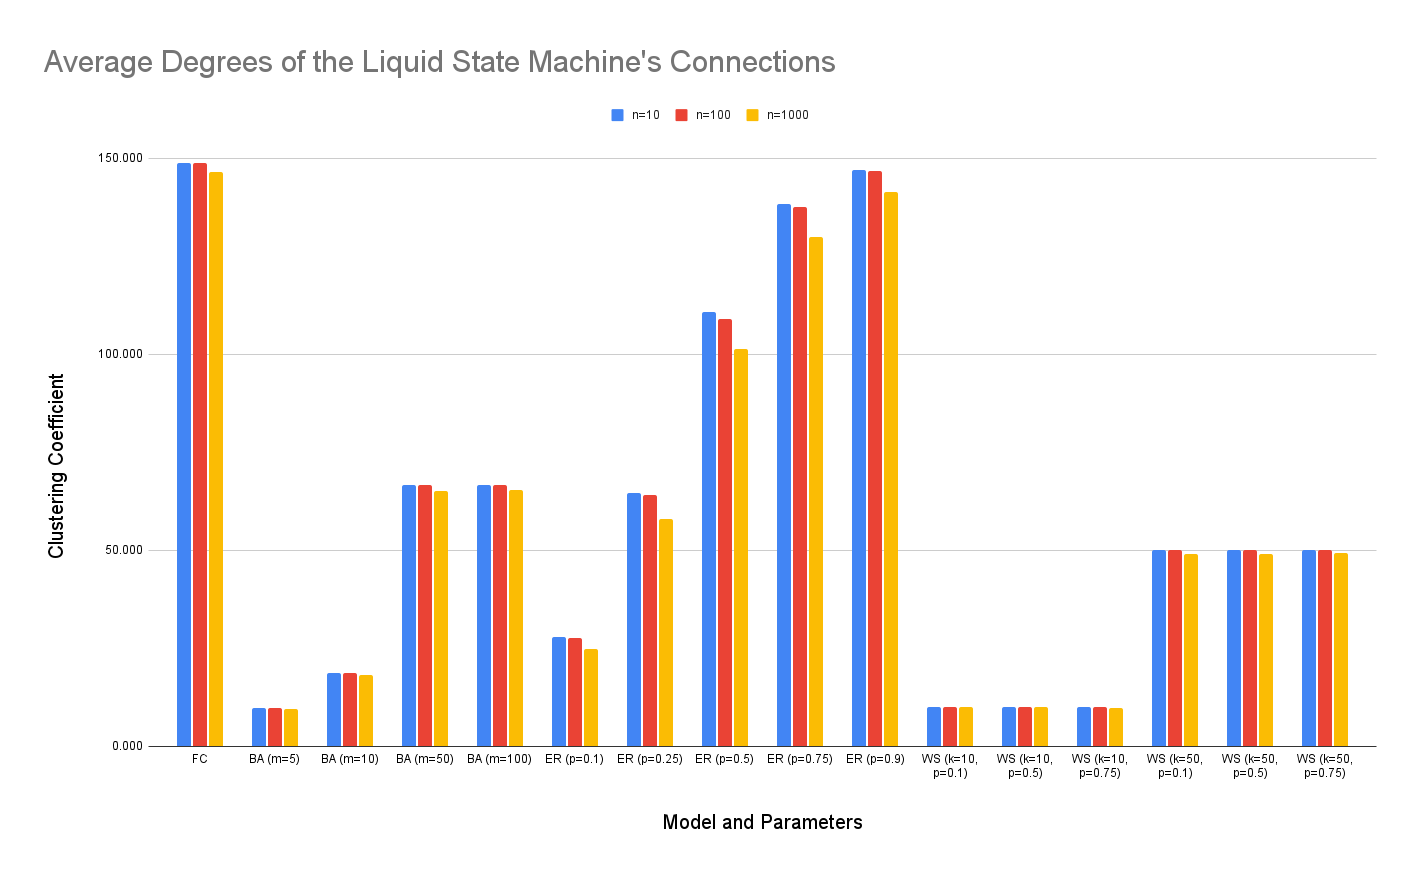
\includegraphics[scale=0.17]{avgDeg.png}
    \caption{
        Average degrees of all networks. The blue bars are $n=10$ samples, the
        red $n=100$, and the yellow $n=1000$.
    }
    \label{fig:avgDeg}
\end{figure}

The important trend here is the decreasing of average degree experienced by all
models. We see this difference exaggerate itself in Erdos-Renyi networks, which
we can further examine in \ref{fig:erAdj0.5}. This finding is more pronounced
in the differences graph in \ref{fig:erAdj0.5Diff}.

\begin{figure}[h]
    \centering
    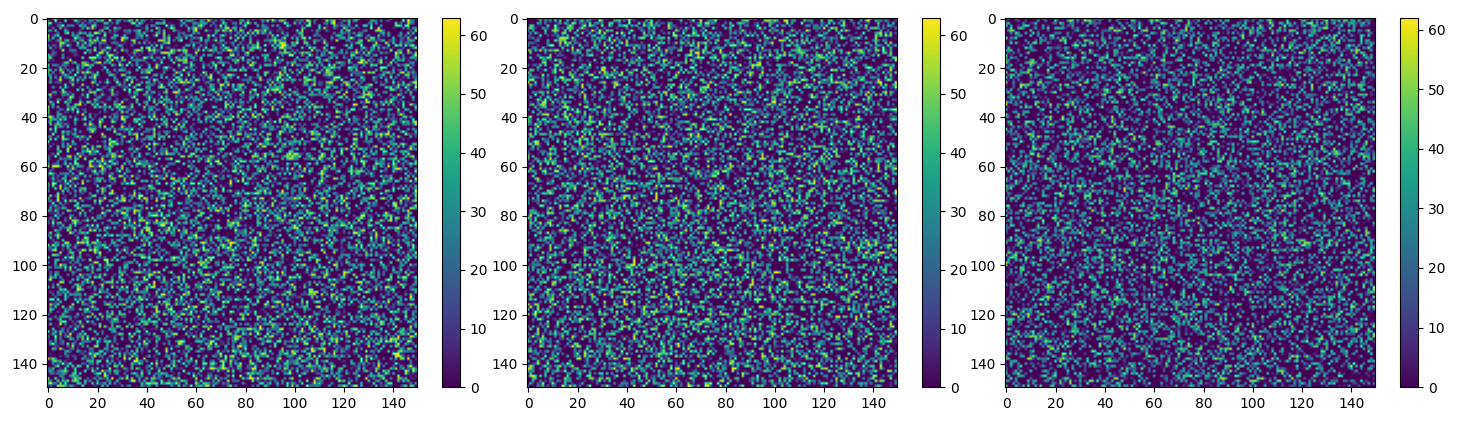
\includegraphics[scale=0.22]{erAdj0.5.png}
    \caption{
        Diagrams of the Erdos-Renyi network's adjacency matrices (with
        connection probability $p=0.5$). The left diagram is at $n=10$ samples,
        the middle at $n=100$ samples, and the right at $n=1000$ samples.
    }
    \label{fig:erAdj0.5}
\end{figure}

\begin{figure}[h]
    \centering
    \includegraphics[scale=0.22]{erAdj0.5Diff.png}
    \caption{
        Diagrams of the Erdos-Renyi network's adjacency matrix differences from
        initial seed configuratons (with connection probability $p=0.5$). The
        left diagram is at $n=10$ samples, the middle at $n=100$ samples, and
        the right at $n=1000$ samples.
    }
    \label{fig:erAdj0.5Diff}
\end{figure}

In particular, Erdos-Renyi suffers from a very high rate of connection removal
with increasing training samples. This is likely due to the extremely high
degree connectivity, which is a feature of this network.

\subsection{The Watts-Strogatz Model}

As shown in \ref{fig:avgDeg}, the Watts-Strogatz model degenerated to extremely
low average degrees over time. In order to see if the model kept its small-world
characteristics, we examined clustering coefficients in \ref{fig:clustering}.

\begin{figure}[h]
    \centering
    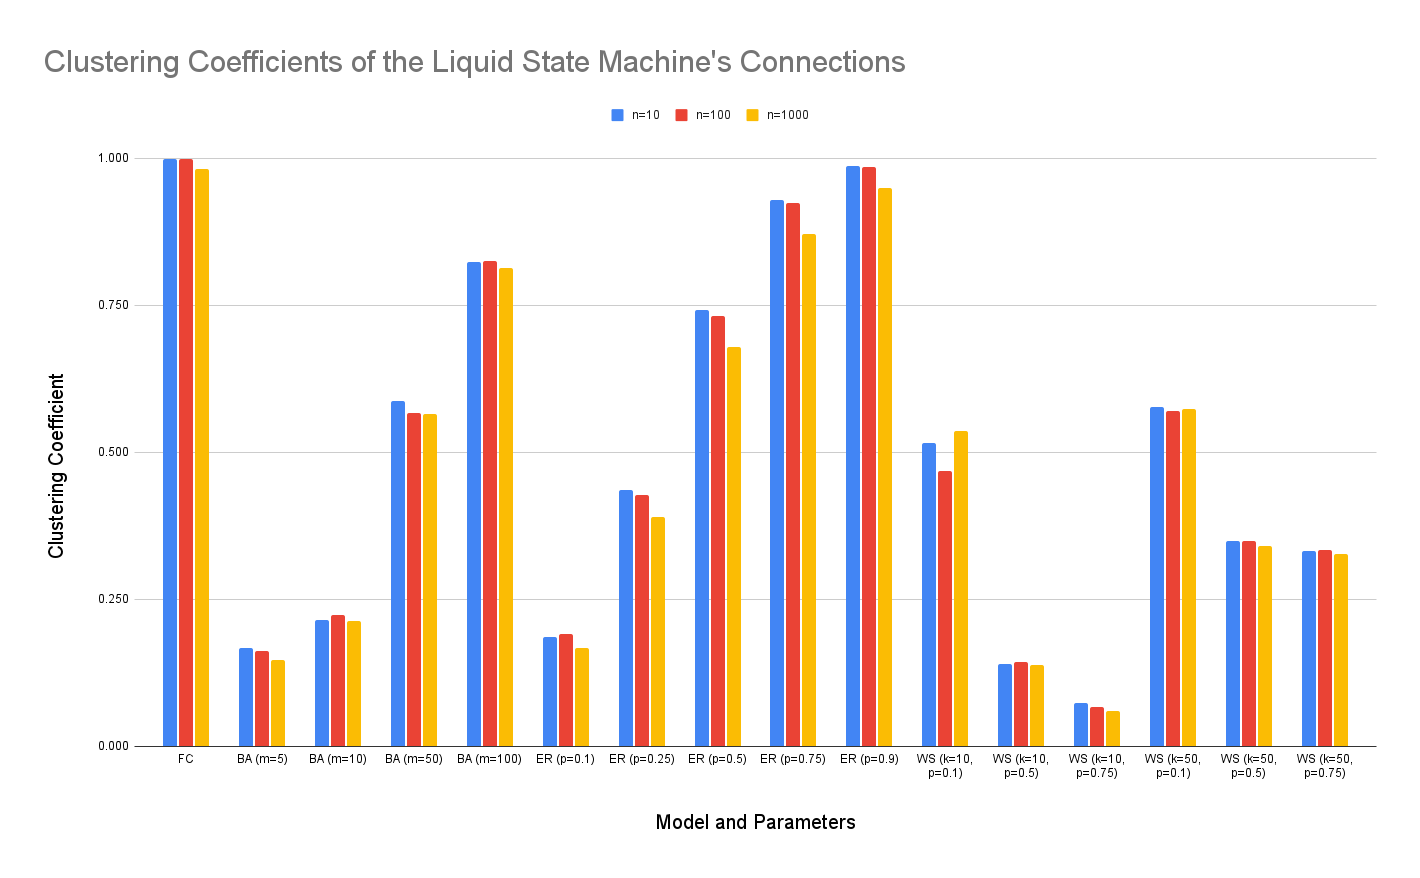
\includegraphics[scale=0.17]{clustering.png}
    \caption{
        Clustering coefficients of all networks. The blue bars are $n=10$
        samples, the red $n=100$, and the yellow $n=1000$.
    }
    \label{fig:clustering}
\end{figure}

We noticed that the Watts-Strogatz models quickly degenerated to extremely low
clustering coefficients, which is in direct contrast to the small-world
principle of having significantly large clustering coefficients when compared
to Erdos-Renyi models. We also looked at the shortest path length, which is a
direct indicator of network diameter, in \ref{fig:path}.

\begin{figure}[h]
    \centering
    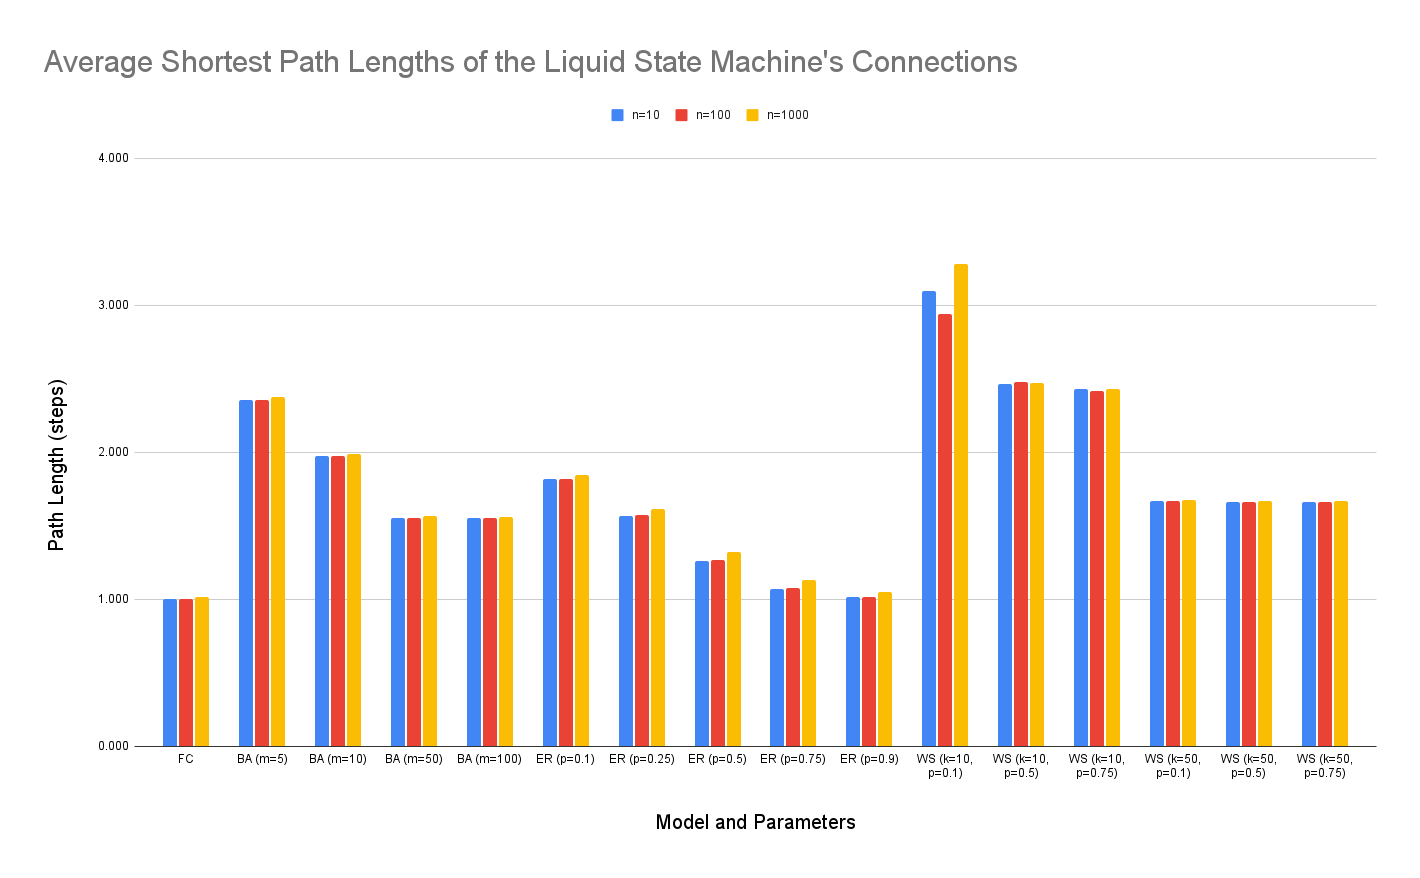
\includegraphics[scale=0.17]{path.png}
    \caption{
        Average shortest path lengths of all networks. The blue bars are $n=10$
        samples, the red $n=100$, and the yellow $n=1000$.
    }
    \label{fig:path}
\end{figure}

Once again we see data in direct contrast to expectation. The small-world
property is defined with small network diameters and large clustering
coefficients. However, we see that STDP training rules degenerate a network into
a very sparse graph with low clustering coefficients and high network diameters.
One interpretation for this is that sparser models are more 'fitting' for data;
This backs up the idea of inhibition being a key to the network, as discussed
in \cite{Astrocyte}. We can see the graph generated in \ref{fig:wsk10p0.75}.

\begin{figure}[h]
    \centering
    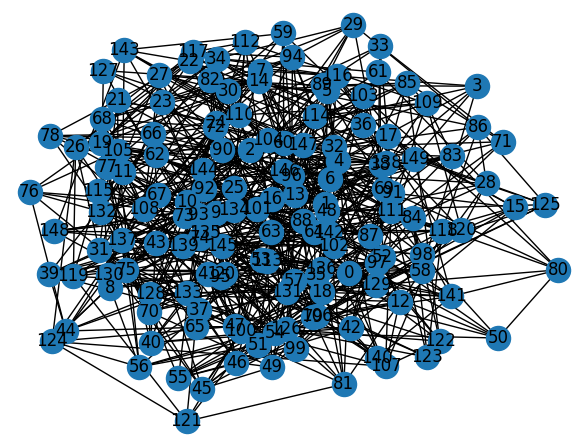
\includegraphics[scale=0.5]{wsk10p0.75.png}
    \caption{
        Diagram of the generated Watts-Strogatz graph with parameters $p=0.75$,
        $k=10$, after training for $n=1000$ samples.
    }
    \label{fig:wsk10p0.75}
\end{figure}

We can further dive into the network's structure by looking at the adjacency
matrices. The adjacency matrix comparison is in \ref{fig:wsk10p0.75Adj}, and the
difference matrix comparison is in \ref{fig:wsDiff}.

\begin{figure}[h]
    \centering
    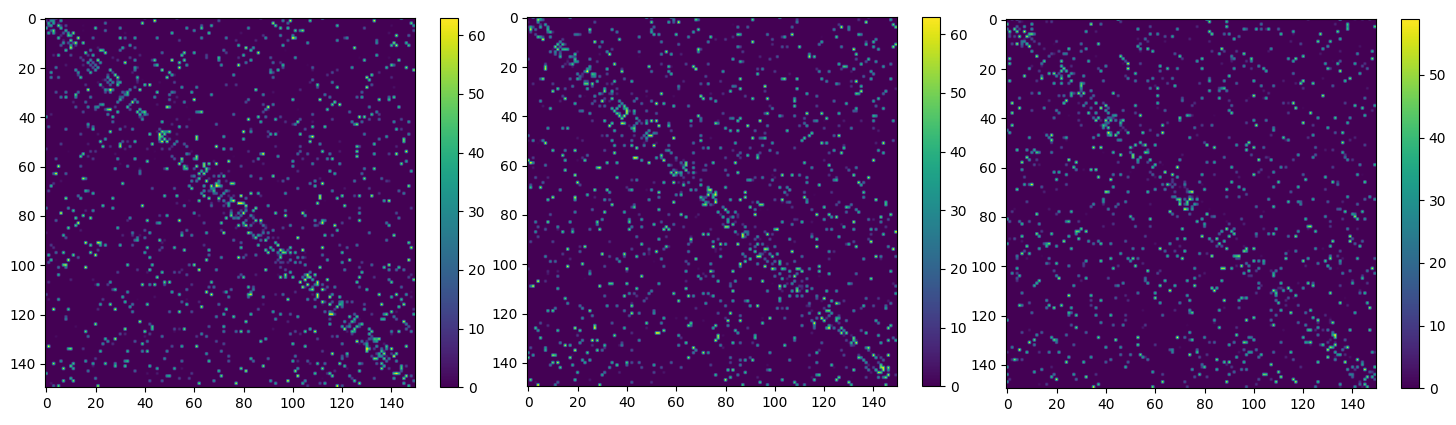
\includegraphics[scale=0.22]{wsk10p0.75adj.png}
    \caption{
        Diagrams of the Watts-Strogatz network's adjacency matrices (with
        $p=0.75$, $k=10$). The left diagram is at $n=10$ samples,
        the middle at $n=100$ samples, and the right at $n=1000$ samples.
    }
    \label{fig:wsk10p0.75Adj}
\end{figure}

\begin{figure}[h]
    \centering
    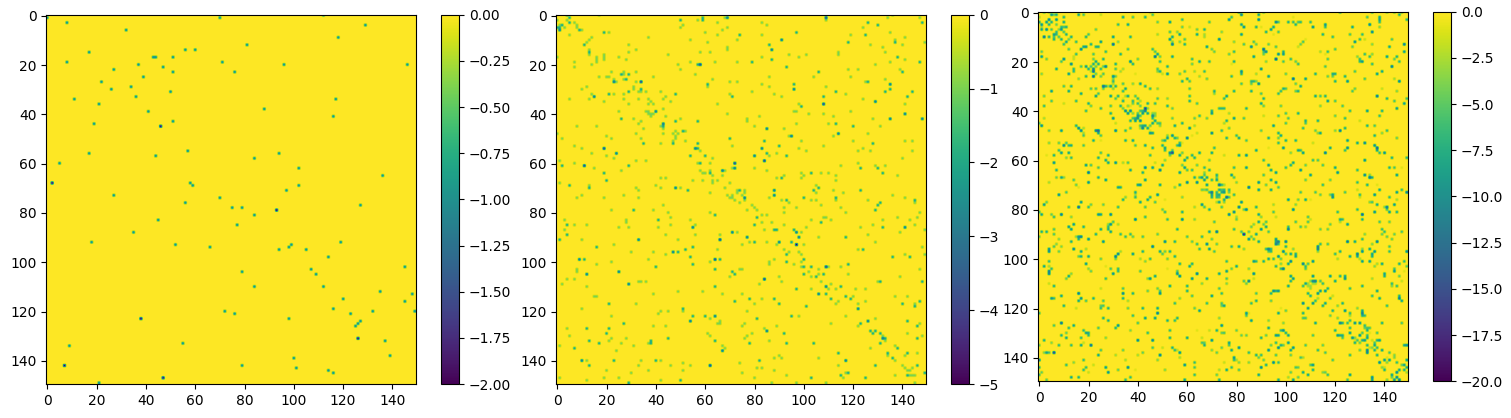
\includegraphics[scale=0.22]{wsDiff.png}
    \caption{
        Diagrams of the Watts-Strogatz network's adjacency matrix differences
        from the initial seed configuration (with $p=0.75$, $k=10$). The left
        diagram is at $n=10$ samples, the middle at $n=100$ samples, and the
        right at $n=1000$ samples.
    }
    \label{fig:wsDiff}
\end{figure}

A significant band of negations forms, indicating that the network is removing
connections in order to reduce clustering coefficient and subsequently increase
path length.

\subsection{Information Walks}

In order to further explore this idea of inhibition being key to the network, we
examined how new information would spread throughout the network through
application of an SI spreading model. Nodes $n_i$ and $n_j$ that have a
corresponding directed weight $w_{ij}$ between them would transmit information
with a probability of $\frac{w_{ij}}{\theta}$. As such, information is
'transmitted' through the network based on the probability that a particular
neuron's excitation causes another neuron to fire. One such information walk is
presented in \ref{fig:wsWalk}.

\begin{figure}[h]
    \centering
    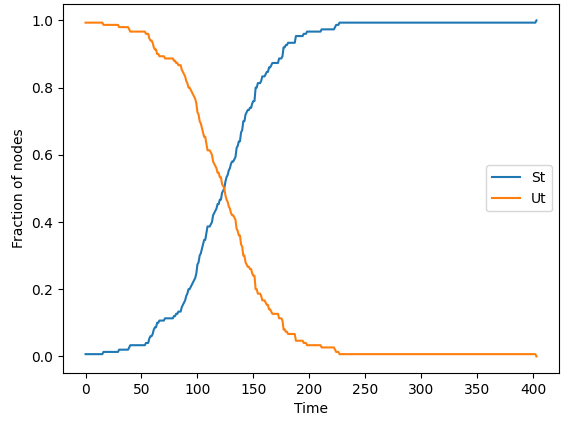
\includegraphics[scale=0.58]{wsWalk.png}
    \caption{
        'Information walk' SI spreading process throughout the Watts-Strogatz
        network trained with $n=10$ samples, with parameters $p=0.75$ and
        $k=10$.
    }
    \label{fig:wsWalk}
\end{figure}

We compiled these results results for all networks, which can be seen in the
graph in \ref{fig:infowalk}.

\begin{figure}[h]
    \centering
    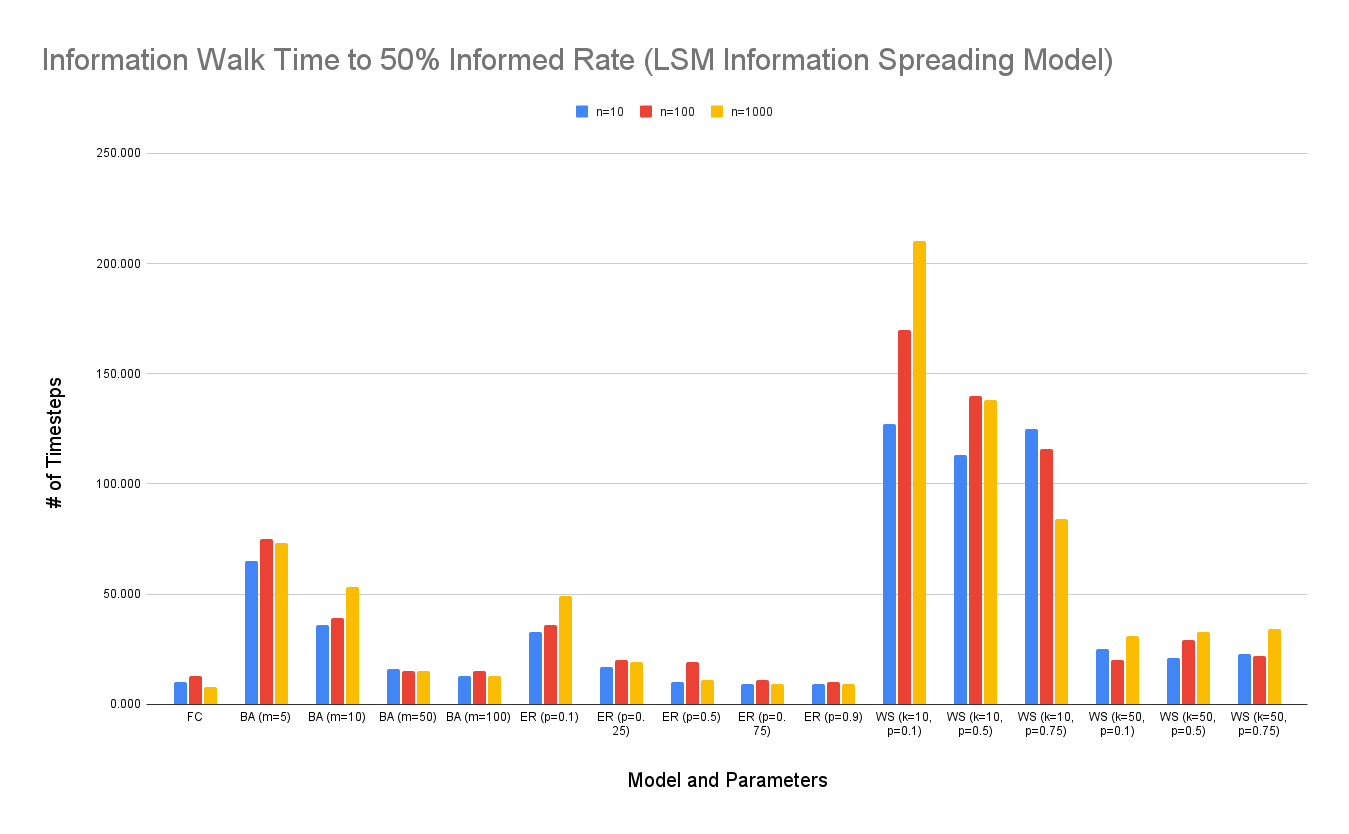
\includegraphics[scale=0.17]{infowalk.png}
    \caption{
        Graph of times to reach 50\% of the nodes in the network for all
        networks. The blue bars are $n=10$ training samples, the red $n=100$,
        and the yellow $n=1000$.
    }
    \label{fig:infowalk}
\end{figure}

As shown in the graph, information walk times experience an extreme spike in
only the Watts-Strogatz models. A real-world interpretation of this comes from
the motivation for astroglia within the neocortex. A lower walk time indicates
that nodes activate more rapidly from new information, which may actually be
poor for a network. Inhibitory cells like astrocytes exist such that the human
brain does not constantly experience seizures or overwrite information. The
neural connections modelled may experience better and more stable firing
patterns when more resilient to incoming input changes.

Another interesting note from this data is how particularly chosen smaller
parameters of Watts-Strogatz models seem to increase information walk time. Some
Barabasi-Albert models come close with extremely low parameter values as well.
Increasing inhibition may end up leading to increased performance with the
network - As the network changes less in response to new information, the output
discriminant column may have a more stable and accurate comparison of inputs to
outputs.

\subsection{Limitations}

The main limitation of this project is scope - In the interest of time, the
sizing of the networks as well as a variety of parameters could not be explored.
Different theoretical models for learning, such as Kheradpisheh et al.'s STDP
model \cite{Kheradpisheh} could also be explored, and it's unknown if the
network degeneration we experienced is a feature of STDP or a feature of the
NCAL implementation of Hebbian theory. This and more is examined in
\ref{sec:Future Work}.